\section{Trigonometric Functions}

\subsection{The Unit Circle}
\begin{frame}
    \frametitle{The Unit Circle}
    \begin{definition}
        The \textbf{unit circle} is the circle in the Cartesian plane with center at the origin and radius 1, defined by the equation:
        \[
        x^2 + y^2 = 1
        \]
    \end{definition}                                                                                                                                    
\end{frame}

\begin{frame}
    \frametitle{Radius corresponding to a positive angle}
    \centering
    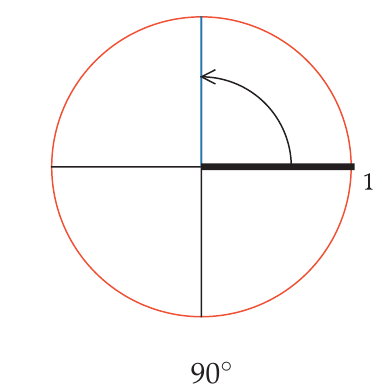
\includegraphics[scale=0.5]{/unit_circle/1.png}
\end{frame}

\begin{frame}
    \frametitle{Radius corresponding to a negative angle}
    \centering
    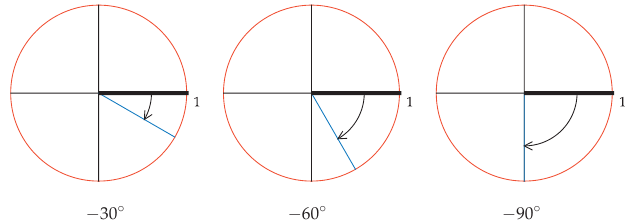
\includegraphics[scale=0.5]{/unit_circle/2.png}
\end{frame}

\begin{frame}
    \begin{block}{Positive and Negative Angles}
        \begin{itemize}
            \item Angle measurements for a radius on the unit circle are made from the positive horizontal axis.
            \item Positive angles correspond to moving counterclockwise from the positive horizontal axis.
            \item Negative angles correspond to moving clockwise from the positive horizontal axis.
        \end{itemize}
    \end{block}
\end{frame}

\begin{frame}
    \frametitle{Angles more than 360 degrees}
    \begin{block}{cyclic behaviour of angles}
        A radius of the unit circle corresponding to $\theta$ degrees also corresponds to $\theta + 360n$ degrees for every integer n.
    \end{block}
    \begin{figure}[h]    
        \centering
        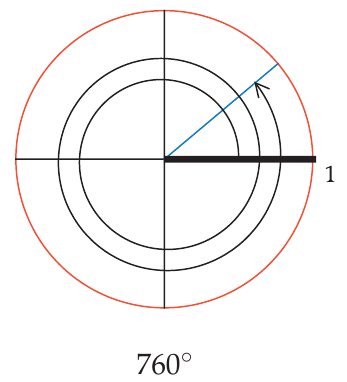
\includegraphics[scale=0.4]{/unit_circle/3.png}
    \end{figure}
\end{frame}

\begin{frame}
    \frametitle{Length of a Circular Arc}
    \begin{figure}
        \centering
        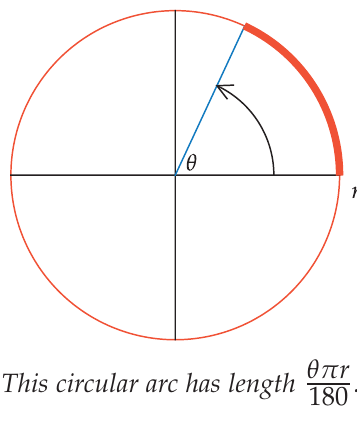
\includegraphics[scale=0.5]{/unit_circle/5.png}
    \end{figure}
    \[ 360^{\circ}   \rightarrow  2 \pi r \implies \theta^{\circ}  \rightarrow \frac{\theta}{360}.2\pi r  = \frac{\theta \pi r}{180}\] 
\end{frame}

\begin{frame}
    \frametitle{Radians}
    For example an ant moving around a unit circle would travel a distance of $2\pi$ radians when it completes one full rotation.
    \begin{block}{Radians}
        Radians are a unit of measurement for angles such that $2\pi$ radians correspond to a rotation through an entire circle.
    \end{block}
\end{frame}

\begin{frame}
    \frametitle{Radians}
    \begin{block}{Degree to Radians}
        \[ 360^{\circ} = 2 \pi \text{ radians} \]
        \[ \theta ^{\circ}  = \frac{\theta \pi}{180} \text{ radians} \]
    \end{block}
\end{frame}

\begin{frame}
    \frametitle{Arc Length}
    \begin{block}{length of a circular arc}
        If $0 < \theta \leq 2\pi$ , then a circular arc on the unit circle corresponding to $\theta$ radians has length $\theta$         
    \end{block}
\end{frame}

\begin{frame}
    \frametitle{Area of a Sector}
    \begin{block}{Area of a sector}
        A sector/slice with angle $\theta$ radians inside a circle with radius $r$ has area $\frac{1}{2} \theta r^{2}$ .
    \end{block}
    \begin{figure}[h]    
        \centering
        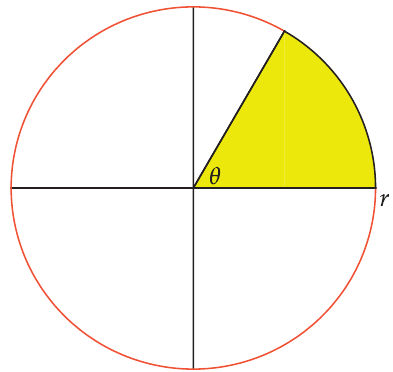
\includegraphics[scale=0.25]{unit_circle/6.png}
    \end{figure}
\end{frame}

\begin{frame}
    \frametitle{Note}
    \begin{block}{Note}
        If no unit is specified, angles are assumed to be in radians.
    \end{block}
\end{frame}

\begin{frame}
    \frametitle{Cosine and Sine}
    \begin{block}{Definitions}
        \begin{itemize}
            \item The \textbf{cosine} of an angle $\theta$ is the x-coordinate of the point on the unit circle corresponding to that angle.
            \item The \textbf{sine} of an angle $\theta$ is the y-coordinate of the point on the unit circle corresponding to that angle.
        \end{itemize}
    \end{block}     
    \begin{figure}[h]    
        \begin{minipage}[b]{0.8\textwidth}
            \centering
            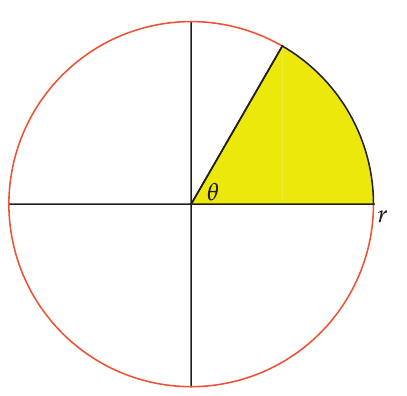
\includegraphics[scale=0.22]{unit_circle/7.png}
            \caption{sine and cosine}
        \end{minipage}
    \end{figure}
\end{frame}

\begin{frame}
    \frametitle{The Signs of Sine and Cosine} 
    \begin{figure}
        \centering
        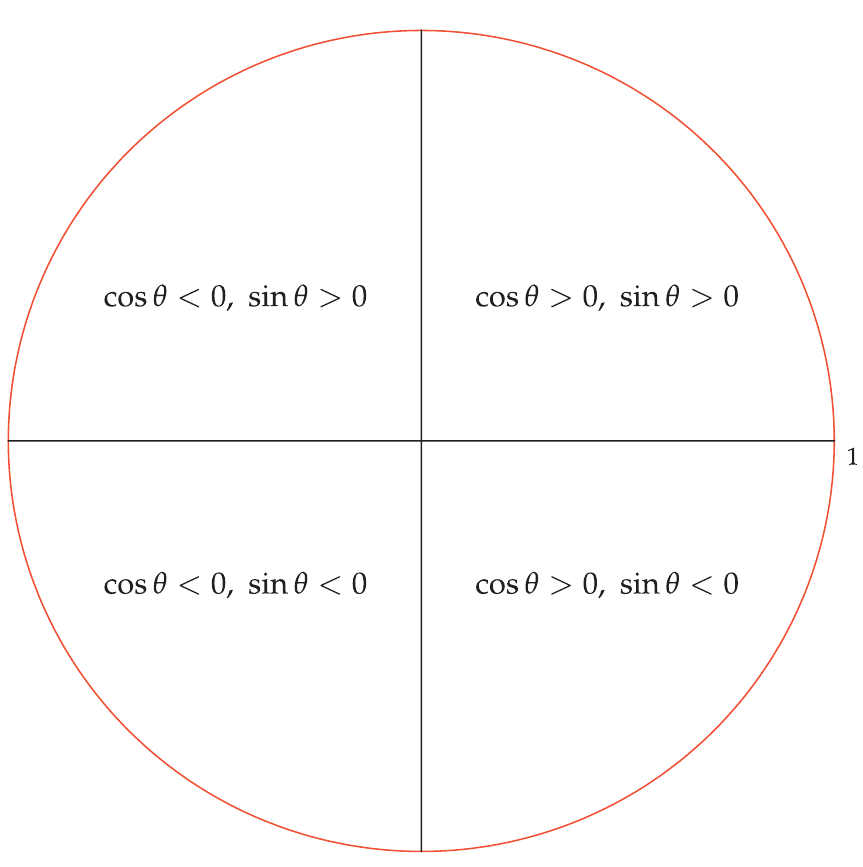
\includegraphics[scale=0.2]{unit_circle/8.png}
        \caption{Signs of sine and cosine in different quadrants}
    \end{figure}
\end{frame}

\begin{frame}
    \frametitle{Key Equation Connecting Sine and Cosine} 
    \begin{itemize}
        \item By definition cosine and sine are the x and y coordinates of a point on the unit circle.
        \item The equation of the unit circle is $x^2 + y^2 = 1$.
        \item Therefore, for any angle $\theta$,
    \end{itemize}
    \begin{block}{Key Identity}
        \[\cos^2(\theta) + \sin^2(\theta) = 1\]
    \end{block}
\end{frame}

\begin{frame}
    \frametitle{The limits of Sine and Cosine} 
    \begin{itemize}
        \item For each real number $\theta$, there is a radius of the unit circle corresponding to that angle.
        \item The co-ordinates of the end point of the radius are $(\cos(\theta), \sin(\theta))$.
        \item That is this function is defined for all real numbers because theta can take any real value. 
        \item The domain of sine and cosine is all real numbers. \(\mathbb{R}\) 
        \item For unit circle \( \cos \theta^{2} + \sin \theta^{2} = 1 \) 
        \item Because \( \cos \theta^{2} + \sin \theta^{2} = 1 \) for all \(\theta\), the range of both sine and cosine is limited to \([-1, 1]\).
    \end{itemize}
\end{frame}

\begin{frame}
    \frametitle{Domain and Range of Sine and Cosine}
    \begin{block}{Cosine and Sine are between -1 and 1}
        \[
        -1 \leq \cos(\theta) \leq 1 \quad \text{and} \quad -1 \leq \sin(\theta) \leq 1
        \] for all \(\theta \in \mathbb{R}\)
    \end{block}
    \begin{block}{Domain and Range}
        \begin{itemize}
            \item Domain of sine and cosine: \(\mathbb{R}\)
            \item Range of sine and cosine: \([-1, 1]\)
        \end{itemize}
    \end{block}
\end{frame}

\begin{frame}
    \frametitle{Tangent}
    \begin{block}{Definition of Tangent}
        The \textbf{tangent} of an angle $\theta$ is defined as the ratio of the sine to the cosine of that angle:
        \[\tan(\theta) = \frac{\sin(\theta)}{\cos(\theta)}\]   
        provided that \(\cos(\theta) \neq 0\).
    \end{block}
\end{frame}

\begin{frame}
    \frametitle{Tangent as Slope}
    \begin{figure}
        \centering
        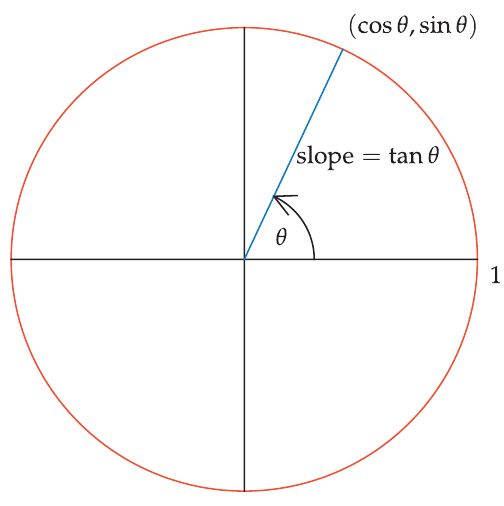
\includegraphics[scale=0.2]{unit_circle/9.png}
        \caption{Tangent as slope of the radius}
    \end{figure}
    \centering
    \[ 
        \text{Slope} = \frac{y_{2} - y_{1}}{x_{2} - x_{1}} = \frac{\sin(\theta) - 0}{\cos(\theta) - 0} = \tan(\theta)
    \]
    \(\tan \theta\) is the slope of the radius corresponding to angle \(\theta\) in the \textbf{unit circle}.
    \textbf{Note:} The slope of the radius applies to any circle, not just the unit circle.
\end{frame}

\begin{frame}
    \frametitle{Sign of Tangent}
    \begin{figure}
        \centering
        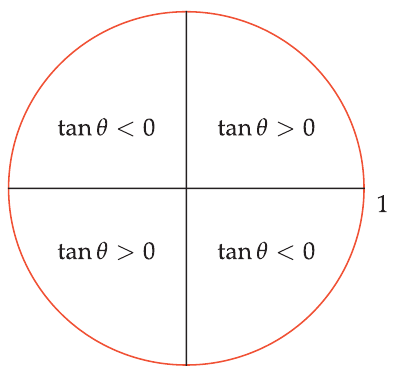
\includegraphics[scale=0.2]{unit_circle/10.png}
        \caption{Signs of tangent in different quadrants}
    \end{figure}
\end{frame}

\begin{frame}
    \frametitle{Radius of unit circle corresponding to a positive angle}
    \begin{figure}
        \centering
        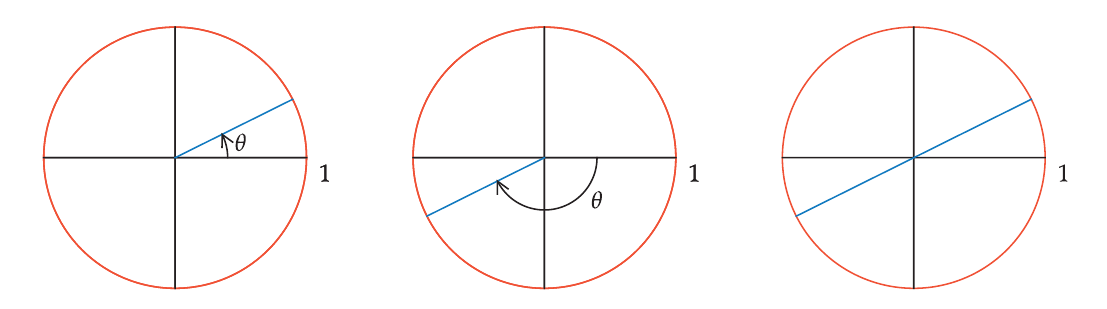
\includegraphics[scale=0.25]{unit_circle/11.png}
        \caption{Radius of unit circle corresponding to angle \(\theta\) such that \(\tan(\theta) = \frac{1}{2}\)}
    \end{figure}
\end{frame}

\begin{frame}
    \frametitle{Domain and Range of Tangent}
    \begin{itemize}
        \item Tangent is defined for all angles except those where \(\cos(\theta) = 0\), which occurs at odd multiples of \(\frac{\pi}{2}\).
        \item The tangent of an angle is the slope of the corresponding radius in the unit circle.
        \item Every real number is the slope of some radius in the unit circle. So range of tangent is all real numbers.
        \item The domain of tangent is all real numbers except odd multiples of \(\frac{\pi}{2}\):
        \[\text{Domain of } \tan(\theta) = \mathbb{R} \setminus \left\{ \theta \mid \theta = \frac{\pi}{2} + n\pi, n \in \mathbb{Z} \right\}\]
        \item The range of tangent is all real numbers:
        \[\text{Range of } \tan(\theta) = \mathbb{R}\]  
    \end{itemize}

\end{frame} 

\begin{frame}
    \frametitle{Graphing Tangent: Tangent near \(\frac{\pi}{2}\)}
    \begin{figure}
        \centering
        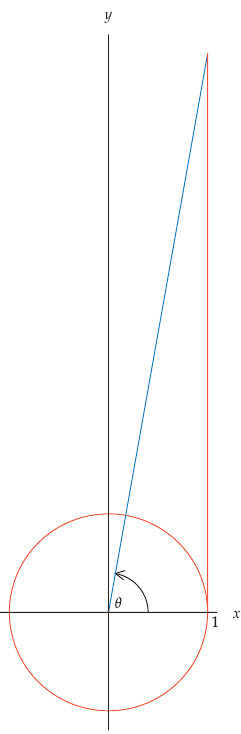
\includegraphics[scale=0.28]{/unit_circle/12.png}
    \end{figure}
\end{frame}

\subsection{Trigonometry in Right Triangles}
\begin{frame}
    \frametitle{Right Triangle Definitions}
    For \(0<\theta<\frac{\pi}{2}\) in a right triangle:
    \begin{itemize}
        \item In a right triangle, the side opposite the right angle is the \textbf{hypotenuse}.
        \item The other two sides are referred to as the \textbf{adjacent} and \textbf{opposite} sides, depending on the angle of interest.
    \end{itemize}
\end{frame}
\begin{frame}
    \frametitle{Right Triangles}
    \begin{figure}
        \centering
        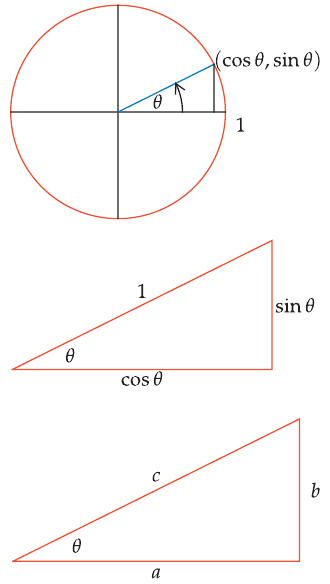
\includegraphics[scale=0.3]{/unit_circle/13.png}
    \end{figure}
\end{frame}

\begin{frame}
    \frametitle{SOH-CAH-TOA}
    \begin{itemize}
        \item \textbf{SOH}: \(\sin(\theta) = \frac{\text{opposite}}{\text{hypotenuse}}\)
        \item \textbf{CAH}: \(\cos(\theta) = \frac{\text{adjacent}}{\text{hypotenuse}}\)
        \item \textbf{TOA}: \(\tan(\theta) = \frac{\text{opposite}}{\text{adjacent}}\)
    \end{itemize}
\end{frame}